% day01.tex

% Copyright 2019 Clara Eleonore Pavillet

% Author: Clara Eleonore Pavillet
% Description: This is an unofficial Oxford University Beamer Template I made from scratch. Feel free to use it, modify it, share it.
% Version: 1.0

\documentclass{beamer}
\setbeamertemplate{caption}[numbered]
\usepackage{import} % for some reason, this doesn't work when called in sty file
% Load Packages
\usepackage[utf8]{inputenc}
\usepackage{xcolor}
\usepackage{tikz}
\usetikzlibrary{positioning,calc}
\usepackage{graphicx}
\usepackage{hyperref}
\usepackage{amsmath}
\usepackage{listings}
\usepackage{fontawesome}

% Define Commands
\newcommand*{\ClipSep}{0.06cm} %To adjust footer logo
\newcommand{\E}{\mathrm{e}\,} %\def\I{e} % used to defined e for exp(x), see later what it should be
\newcommand{\ud}{\mathrm{d}}
\lstset{numbers=left, numberstyle=\tiny, stepnumber=1,firstnumber=1,breaklines=true,
    numbersep=5pt,language=Python,
    stringstyle=\ttfamily,
    basicstyle=\footnotesize, 
    showstringspaces=false
}

\usepackage{lecture_notes}
\usepackage{bibentry}
\usepackage[utf8]{inputenc}
\usepackage[T1]{fontenc}

\graphicspath{ {images/} }

\nobibliography*
% \usepackage[perpage]{footmisc}
\usetheme{oxonian}


\title{Day 01: Intro to \LaTeX }
\titlegraphic{
\includegraphics[width=3cm]{Theme/Logos/DavisLogoV1.png}}
\author{\small{Mason del Rosario}}
\institute{\LaTeX 101}
\date{September 2021} %\today

\begin{document}

\footnotesize{
% \bibliographystyle{ieeetr}
% \nobibliography*{refs}


{\setbeamertemplate{footline}{} 
\frame{\titlepage}}

\section*{Outline}\begin{frame}{Outline}\tableofcontents\end{frame}

\section{Introduction}

  % Introduction section frame 
  \begin{frame}[plain]
    \vfill
    \centering
    \begin{beamercolorbox}[sep=8pt,center,shadow=true,rounded=true]{Background}
      \usebeamerfont{title}\insertsectionhead\par%
      \color{davisblue}\noindent\rule{10cm}{1pt} \\
      \footnotesize{Course Background}
    \end{beamercolorbox}
    \vfill
  \end{frame}
  
\subsection{Course Background}

  \begin{frame}{Course Background}
    \begin{itemize} 
      \item \textbf{Inspiration} -- https://www.learnlatex.org/. 
      \item \textbf{Slides Available} -- https://github.com/mdelrosa/latex-101.
      \begin{itemize}
        \item Template based on \href{https://www.overleaf.com/latex/templates/oxpav/xnjgrxthvjhg}{Clara Pavillet's Oxford Template}
      \end{itemize}
      \item \textbf{Slack back channel}
      \begin{itemize}
        \item \href{https://join.slack.com/share/zt-ul82okyc-SI2GftuwPx_lFyBXll9rjw}{UC Davis Slack channel}
      \end{itemize}
    \end{itemize}
  \end{frame}

\subsection{What is \LaTeX?}

  \begin{frame}{Markup Language}
    \textbf{Markup Language} -- Instructions for rendering a document.
    \begin{figure}
      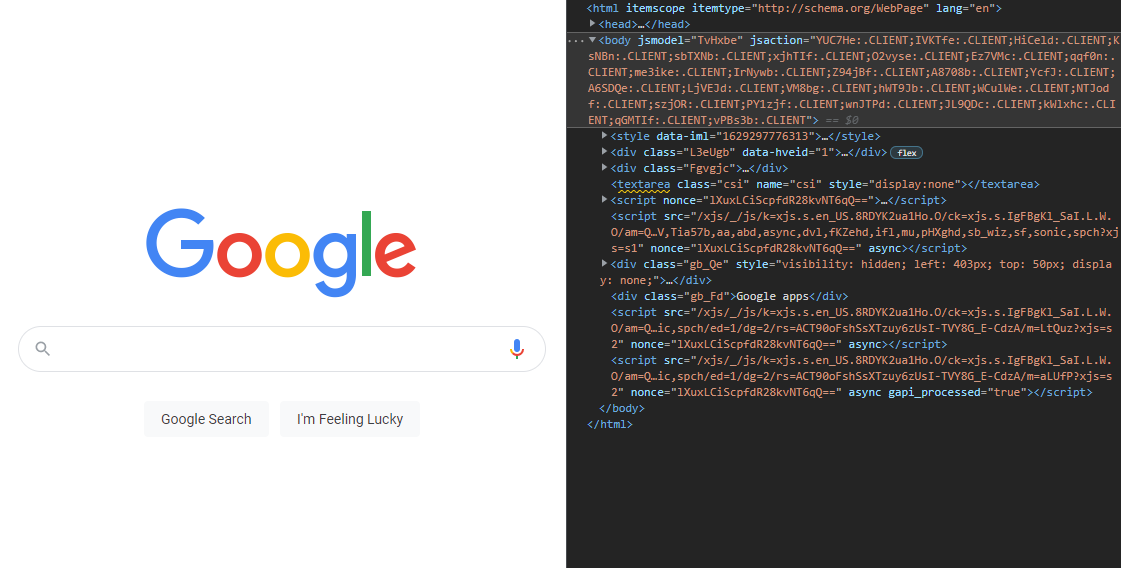
\includegraphics[width=0.8\linewidth]{google_html.png}
      \caption{Example -- HTML for websites}
      \label{fig:html}
    \end{figure}
  \end{frame}

  \begin{frame}{What is \LaTeX?}
    \LaTeX -- Markup language for academic documents (e.g., publications, presentations, lecture notes, assignments).
    \begin{figure}
      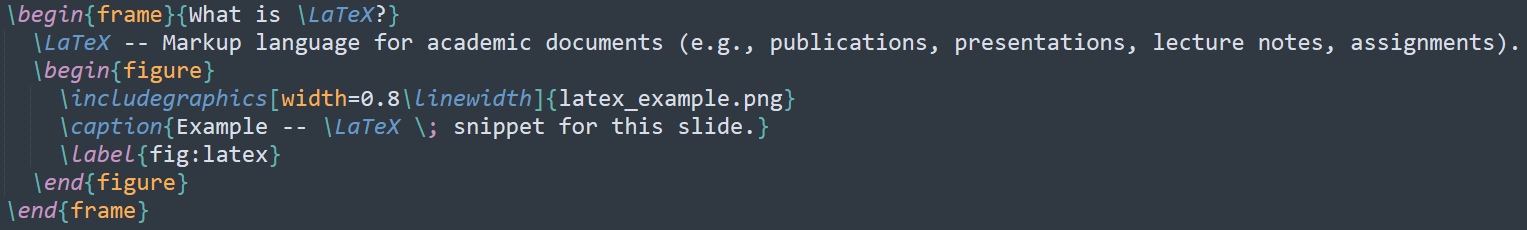
\includegraphics[width=0.8\linewidth]{latex_example.png}
      \caption{Example -- \LaTeX \; snippet for this slide.}
      \label{fig:latex}
    \end{figure}
  \end{frame}


  % show some examples
  % equations, cross-references, citations, figures, and tables of contents
  \begin{frame}{Equations in \LaTeX}
    \begin{equation}
      V_s = \int_{-R}^R \pi (R^2 - x^2) dx = \frac{4}{3}\pi R^3 \label{eq:sphere}
    \end{equation}
    \begin{figure}
      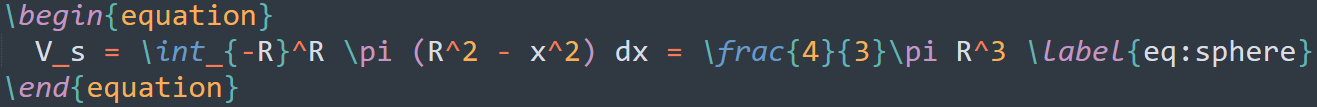
\includegraphics[width=0.8\linewidth]{equation_example.png}
      \caption{Example -- \LaTeX snippet for this equation.}
      \label{fig:equation}
    \end{figure}
  \end{frame}

  \begin{frame}{Cross-references in \LaTeX}
    Enables rich cross-referencing of equations, figures, tables
    \begin{itemize}
      \item Equation \ref{eq:sphere} (previous page)
      \item Table \ref{tab:ex-table} 
    \end{itemize}
    \begin{table}
      \centering
      \begin{tabular}{c|c}
        \textbf{Feature} & \textbf{Support} \\ \hline
        Figures & Yes! \\ \hline
        Equations & Yes! \\ \hline
        Tables & Yes! \\ \hline
        Bibliographies & Yes! \\ 
      \end{tabular}
      \caption{A simple table.}
      \label{tab:ex-table}
    \end{table}
  \end{frame}

  \begin{frame}{How does \LaTeX work?}
    Two primary components/steps:
    \begin{enumerate}
      \item Write your \LaTeX file(s) (\textbf{Text editor})
      \item ``Compile'' or ``Typeset'' your document (\textbf{\LaTeX \;system})
    \end{enumerate}
    \vspace{0.125in}
    \begin{figure}
      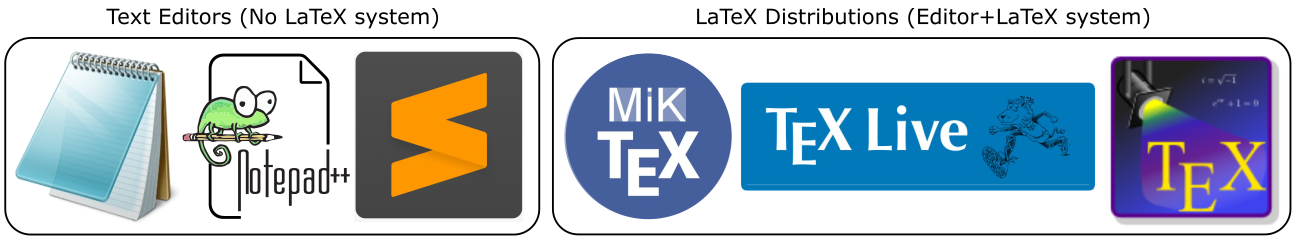
\includegraphics[width=0.8\linewidth]{tex_systems.png}
      \caption{Text editors (Notepad, Notepad++, Sublime Text) and LaTeX distributions (MikTeX, TeXLive, and TeX Studio)}
      \label{fig:systems}
    \end{figure}
  \end{frame}

  \begin{frame}{\LaTeX in this course}
    \begin{itemize}
      \item Editors/systems installed on local device (faster, private)
      \pause
      \item Editor/systems online (convenient, collaborative)
      \pause
      \item Will use \textbf{Overleaf} for this course.
    \end{itemize}
    \begin{figure}
      
\includegraphics[width=0.6\linewidth]{overleaf.png}
    \end{figure}
  \end{frame}

  \section{\LaTeX Document Structure}

} %end footnotsize
\end{document}
